\section{Thickness and size of the shield}\label{sec:5:shield-size}
The thickness $d$ and the radius $r_s$ of the spherical shield can be estimated by considering the properties of a physical conductive material with high electrical conductivity $\sigma$.
Even a superconducting shield could be considered for an almost perfect shielding of electromagnetic fields.
The transmission $T$ of electromagnetic waves through a physical shield is given by \cite{Vandenbosch_2022}
\begin{equation}
  T = \abs{\frac{\vec{E}_\mathrm{after}}{\vec{E}_\mathrm{before}}} = \frac{2}{Z_0 \sigma d}
\end{equation}
where $Z_0 = 377\si{\Omega}$ is the impedance of free space (assuming the shield is placed in a vacuum or in air).
The electric conductivity $\sigma$ is highly dependent on the temperature \cite[p. 284-286]{Gross_2018}, decreasing approximately with $1/T^5$ at low temperatures \footnote{This behavior is valid for temperatures below the Debye temperature ($\Theta_D = 343\si{K}$ for copper). At the low temperatures used in the experiment, this model accurately describes the conductivity of metals \cite{Berman_1952}.}.
Copper offers a strong electric conductivity of $\sigma = 59.6\times 10^6 \si{S/m}$ at room temperature and measured data showing even $\sigma(T = 10\si{K}) \approx 1.5\times 10^{10}\si{S/m}$ at $10\si{K}$ \cite{Berman_1952}.

To estimate the shield's thickness, the primary criterion used, is that gravitational interactions should dominate the entanglement generation.
Other mutual interactions between the particles, such as Coulomb or Casimir forces, must be sufficiently suppressed by the shield.
The \emph{entanglement rate} $\Gamma$ quantifies the build-up of entanglement over time
\begin{equation}\label{eq:5:entanglement-rate}
  \Gamma = \dv{t} E_N(\rho)\Big|_{t=0} \, ,
\end{equation} 
where $E_N$ is an appropriate entanglement measure - in this case the logarithmic negativity \cite{Plenio_2005} introduced in \cref{sec:2:entanglement-measures}.
For gravitational interactions, the entanglement rate in the parallel orientation is given by using eq. \eqref{eq:2:entanglement-dynamics-parallel} as
\begin{equation}\label{eq:5:entanglement-rate-gravity}
  \Gamma_\mathrm{Gravity} = \frac{G M_A M_B \Delta x_A \Delta x_B}{16 \hbar L^3 \log 2} = \frac{G \pi^2 R^6 \rho_\mathrm{Silica}^2 (\Delta x)^2}{9 \hbar L^3 \log 2} .
\end{equation}
where in the last step $M_A = M_B = 4/3 \pi R^3 \rho_\mathrm{Silica}$ and $\Delta x_A = \Delta x_B \equiv \Delta x$ was used.
The entanglement rate for non-gravitational interactions, such as Coulomb or Casimir forces, must be significantly smaller than the gravitational entanglement rate, ideally by a factor $\chi > 1$.
This ensures that the measured entanglement is primarily due to gravitational interactions.
In the following sections, estimations about the thickness and size of the shield are made, to effectively screen Coulomb and Casimir forces.


\subsection{Shielding Coulomb-Interactions}
The primary role of the Faraday shield is to block electromagnetic interactions between particles.
Experimentally, it may be beneficial for the particles to carry a small amount of charge, enabling the use of electrostatic traps with high trapping strength and large controllability \cite{GonzalezBallestero_2021}. 
The Coulomb interaction potential between two charged particles is given by
\begin{equation}
  V = \frac{1}{4\pi\varepsilon_0} \frac{q_A q_B}{2L}
\end{equation}
where $\varepsilon_0 = 8.8542\times 10^{-12}\si{A^2 s^4 m^{-3} kg^{-1}}$ is the permittivity of free space and $\abs{q_{A(B)}} = e = 1.6022\times 10^{-19}\si{C}$ the charge of particle $A$ and $B$ respectively.
This interaction mimics the form of the gravitational potential and can similarly induce entanglement with a entanglement rate
\begin{equation}\label{eq:5:entanglement-rate-coulomb}
  \Gamma_\mathrm{Coulomb} = \frac{T \abs{q_A q_B} (\Delta x)^2}{64 \pi \varepsilon_0 \hbar L^3 \log 2} .
\end{equation}
The shield suppresses the coupling by a factor of $T$.
Requiring $\Gamma_\mathrm{Gravity} > \chi \Gamma_\mathrm{Coulomb}$, the minimum thickness of the shield can be calculated as
\begin{align}\label{eq:5:coulomb-gravity-condition}
  T \frac{\abs{q_A q_B}}{64 \pi \varepsilon_0} \chi \, &< \, \frac{G \pi^2 R^6 \rho_\mathrm{Silica}^2}{9} \\
  \Longleftrightarrow \quad\quad\quad\quad d \, &> \, \frac{9}{32}\frac{1}{Z_0 \sigma} \frac{1}{\pi^3 \varepsilon_0 G \rho_\mathrm{Silica}^2} \frac{e^2}{R^6} \chi .
\end{align}
The thickness strongly depends on the particles size $R$, and large or heavy particles will favor gravitational entanglement generation.
Assuming the particles are silica nano-spheres with parameters given in \cref{tab:paramters}, a minimum shield-thickness of $d \approx 10\si{nm}\chi$ at $4\si{K}$ and of $d \approx 2.5\si{\mu m}\chi$ at room temperature is required.
At low temperatures, a realistic shield thickness could therefore be $d=100\si{nm}$, balancing engineering practicality and electromagnetic suppression.
Exact estimations however depend on the realization of the experiment as well as the precision in which the evolved state is measurable.

Electrostatic fields still can propagate around the finite-sized Faraday shield and potentially induce entanglement.
It is possible to estimate the required shield radius $r_s$ to block a specific amount $\eta$ of the electric field (see \cref{apx:blocking-of-the-shield}):
\begin{equation}\label{eq:5:shield-effectiveness}
  \frac{r_s}{L} = \sqrt{\frac{1-(1-\eta)^2}{(1-\eta)^2}}
\end{equation}
The results are visualized in \cref{fig:5:shield-radius}.
\begin{figure}[!ht]
  \centering
  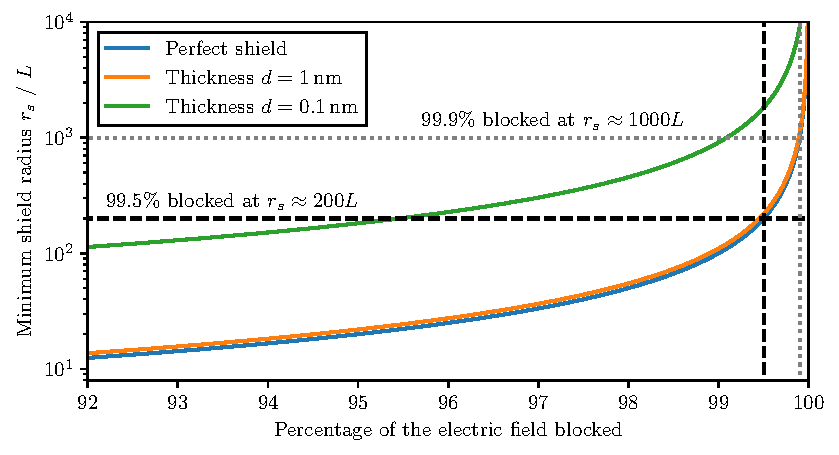
\includegraphics[width=\textwidth]{./../figures/others/shield-radius.pdf}
  \caption{Shield radius as a function of the shielding effectiveness $\eta$ for an ideal shield. Additionally, a real shield with varying thicknesses $d$ is considered at $T=300\si{K}$.
  To achieve shielding of $99.5-99.9\%$ ($\eta = 0.995-0.999$), a radius of $r_s =200-1000L$ is needed.}
  \label{fig:5:shield-radius}
\end{figure}
The shield's transmission $T$ should therefore be modified to $\tilde{T} = T\eta + (1-\eta)$, where the shielding effectiveness $\eta$ depends on $r_s$ as given by eq. \eqref{eq:5:shield-effectiveness}.
Modifying eq. \eqref{eq:5:coulomb-gravity-condition}, a minimum effectiveness $\eta_\mathrm{min}$ for sufficient shielding of
\begin{equation}
  \eta_\mathrm{min} \approx 1 - \frac{64\pi^3 \varepsilon_0 G R^6 \rho^2_\mathrm{Silica}}{9 e^2}
\end{equation}
can be approximated.
Using again the parameters from \cref{tab:paramters}, a minimum shielding of $\eta_\mathrm{min} \gtrsim 0.99997$ and thus a radius of $r_s \gtrsim 28000 L \approx 60\si{cm}$ is required.
Such a shield is too large for all practical purposes and it might be beneficial to choose heavier masses ($\tilde{M} \sim 4 M$) to reduce the shield size to the orders of $\sim 1\si{cm}$.
Due to practicality, a shield with $r_s = 1\si{cm}$ is used in the following calculations.
Uncharged particles would eliminate the Coulomb interactions and therefore reducing the shield's size and thickness to only shield mutual Casimir interactions.




\subsection{Shielding Casimir-Interactions}
Similarly to Coulomb interactions, it is possible to to estimate the required thickness for a shield to sufficiently block Casimir interactions.
The Casimir potential between the spheres with radius $R$ separated by $2L$ is given by \cite{Emig_2007}
\begin{equation}
  V = -\frac{23 \hbar c}{4\pi \cdot 128 L^7} \left( \frac{\varepsilon_r - 1}{\varepsilon_r + 2} \right)^2 R^6 .
\end{equation}
The corresponding entanglement rate is calculated similar to before by expanding the potential in small $\Delta x$ and computing the logarithmic negativity:
\begin{equation}
  \Gamma_\mathrm{Casimir} = T^2 \frac{161}{4096} \frac{c R^6 (\Delta x)^2}{\pi L^9 \log 2}\left( \frac{\varepsilon_r - 1}{\varepsilon_r + 2}\right)^2 .
\end{equation}
The dependence on $T^2$ arises because Casimir forces are second order effects in the dipole-dipole interaction \cite{Bordag_2001}.
Requiring gravitational entanglement generation to dominate, $\Gamma_\mathrm{Gravity} > \chi \Gamma_\mathrm{Casimir}$, leads to
\begin{align}
  T^2 \frac{161 c R^6}{4096 \pi L^6} \left( \frac{\varepsilon_r - 1}{\varepsilon_r + 2}\right)^2 \chi \, &< \, \frac{G \pi^2 \rho_\mathrm{Silica}^2 R^6}{9\hbar} \\
  \Longleftrightarrow \quad\quad\quad\  d \, &> \, \sqrt{\frac{1449}{4096} \frac{c \hbar}{G \pi^3}} \frac{2}{Z_0 \sigma \rho L^3} \frac{\varepsilon_r - 1}{\varepsilon_r + 2} \sqrt{\chi} .
\end{align}
For large separations, the shield thickness can be arbitrarily low, as Casimir forces vanish and at separations of $L\gtrsim 100\si{\mu m}$, the shield might not be required at all (compare \cref{sec:2:experimental-problems}).
Assuming two identical silica nano-spheres with parameters given by \cref{tab:paramters}, the required minimum thickness is between $4\times 10^{-11}\si{m} \sqrt{\chi}$ at $4\si{K}$ and $10 \si{nm} \sqrt{\chi}$ at room temperature.
This is much thinner than what is required for shielding Coulomb interactions.
The factor $\varepsilon_r$ modifies the thickness only by up to a constant factor of $\leq 1$ and is therefore ignored for worst-case estimations.

However, very thin shields lose mechanical rigidity, leading to enhanced vibrational excitations and potential instabilities.
Vibrational frequency and thus the vibrational energy depends linearly on the shield's thickness, making thinner shields prone to large decoherence due to thermal vibrations.
A detailed analysis of these effects is provided in the subsequent section.



\subsection{Gravitational effects of the shield}\label{subsec:5:shield-gravitation}
The gravitational interaction between the masses and the shield is generally neglected because it has no significant impact on the entanglement generation between the particles.
The only potential effect is indirect entanglement mediated by the thermal oscillations of the shield, as both masses couple gravitationally to it. 
However, as shown in \cref{sec:5:thermal-entanglement}, this second-order effect is very weak and does not pose a problem, since it still represents gravitationally mediated entanglement - which is the focus of the experiment anyway.
The gravitational force between a sphere with mass $M$ and an infinitesimal mass segment $\dd m = r d \rho_\mathrm{Cu} \dd r \dd \varphi$ of the shield made of copper with density $\rho_\mathrm{Cu} = 8960\si{kg/m^3}$ at a distance $r$ from the shield's center is given by
\begin{equation}
  \dd \vec{F} = \frac{G M \dd m}{\ell} \boldsymbol{\hat{\ell}} 
  \quad \Rightarrow \quad
  \dd F_z = \frac{G M r \rho_\mathrm{Cu} d}{\ell^2} \dd r \dd \varphi \cos \theta,
\end{equation}
where $\ell^2 = r^2 + L^2$ denotes the distance between the sphere and the mass segment and $\theta = \arccos L/\ell$ is the angle between them.
The total attractive force between the mass and the shield with radius $r_s$ is therefore
\begin{equation}
  F_z = GM \rho_\mathrm{Cu} d L \int\limits_{0}^{r_s} \dd r \int\limits_{0}^{2\pi} \dd \varphi \, \frac{r}{(r^2 + L^2)^{3/2}} = 2\pi G M \rho_\mathrm{Cu} d \left(1 - \frac{L}{\sqrt{L^2 + r_s^2}}\right) .
\end{equation}
For large shields $r_s \gg L$ this is independent of the particle-shield separation $L$.
For a shield with thickness $d = 100\si{nm}$ and the usual silica particle from \cref{tab:paramters}, the attraction force is around $F_\mathrm{particle-shield} \approx 4.1\times 10^{-24} \si{N}$ which is comparable with the attraction gravitational attraction force between the two particles themselves at $F_\mathrm{particle-particle} \approx 5.0 \times 10^{-24}\si{N}$ but is much weaker than the Casimir attraction between the particle and the shield with $F_\mathrm{Casimir} \approx 1.4 \times 10^{-17} \si{N}$.
Therefore, the gravitational effect of the shield can be neglected in all practical calculations.